\documentclass[a4paper,12pt,oneside]{report}

% ------------------------------------------------
% LANGUAGE & FONTS
% ------------------------------------------------
\usepackage[british]{babel}
\usepackage[T1]{fontenc}
\usepackage[utf8]{inputenc}
\usepackage{newtxtext,newtxmath} % Times New Roman-like fonts for pdflatex

% ------------------------------------------------
% PAGE GEOMETRY
% ------------------------------------------------
\usepackage[a4paper,
    left=3.5cm,
    right=1.25cm,
    top=2.5cm,
    bottom=1.25cm
]{geometry}

% ------------------------------------------------
% LINE SPACING & INDENTATION
% ------------------------------------------------
\usepackage{setspace}
\doublespacing
\setlength{\parindent}{1.25cm}

% ------------------------------------------------
% CHAPTER, SECTION, SUBSECTION FORMATTING
% ------------------------------------------------
\usepackage{titlesec}
% Chapter Title - 16pt, Bold, Capital, Centered
\titleformat{\chapter}[block]
  {\centering\normalfont\bfseries\fontsize{16}{20}\selectfont}
  {CHAPTER \thechapter.}{1em}{\MakeUppercase}

% Section - 14pt, Bold
\titleformat{\section}
  {\normalfont\bfseries\fontsize{14}{16}\selectfont}{\thesection}{1em}{}

% Subsection - 12pt, Bold
\titleformat{\subsection}
  {\normalfont\bfseries\fontsize{12}{14}\selectfont}{\thesubsection}{1em}{}

% ------------------------------------------------
% CAPTION SETTINGS
% ------------------------------------------------
\usepackage{caption}
\captionsetup[figure]{
    font={it,small},
    labelfont={bf},
    labelsep=period,
    justification=centering,
    name=Figure
}
\captionsetup[table]{
    font={it,small},
    labelfont={bf},
    labelsep=period,
    justification=centering,
    name=Table,
    position=top
}

% ------------------------------------------------
% NUMBERING FORMAT
% ------------------------------------------------
\numberwithin{equation}{chapter}
\numberwithin{figure}{chapter}
\numberwithin{table}{chapter}

% ------------------------------------------------
% OTHER PACKAGES
% ------------------------------------------------
\usepackage{graphicx}
\usepackage{amsmath}
\usepackage{listings}
\usepackage{float}
\usepackage{makeidx}
\usepackage{hyperref}
\usepackage{xcolor}
\usepackage{microtype}

\lstset{
    basicstyle=\ttfamily\footnotesize,
    breaklines=true
}

% ------------------------------------------------
% TITLE PAGE
% ------------------------------------------------
\begin{document}

\pagenumbering{roman}
\setcounter{page}{1}

\begin{titlepage}
\begin{center}
    \Large\textbf{A REPORT OF FOUR WEEK TRAINING}\\[3mm]
    \large{at}\\[3mm]
    \Large\textbf{Academic Advancement of Information Technology, Mohali}\\[6mm]
    \normalsize{SUBMITTED IN PARTIAL FULFILLMENT OF THE REQUIREMENTS FOR THE AWARD OF DEGREE OF}\\[3mm]
    \Large\textbf{BACHELOR OF TECHNOLOGY}\\[3mm]
    \large{in Computer Science and Engineering}\\[9mm]
    
\includegraphics[height=6cm]{gndeclogo.png}\\[6mm]
    \large{JUNE–JULY 2025}\\[9mm]
    \textbf{SUBMITTED BY:}\\
    NAME: Ayush Mehta\\
    UNIVERSITY ROLL NO.: 2302489
\end{center}

\vspace{10mm}
\begin{center}
    \textbf{Department of Computer Science and Engineering}\\
    \textbf{Guru Nanak Dev Engineering College}\\
    \textbf{Ludhiana, 141006}
\end{center}
\end{titlepage}

% ------------------------------------------------
% CERTIFICATE PAGE (TO BE INSERTED FROM COMPANY)
% ------------------------------------------------
\newpage
\begin{center}
    \large\textbf{CERTIFICATE}\\[6mm]
    
\includegraphics[width=\textwidth, keepaspectratio]{certificate.jpg}
\end{center}

% ------------------------------------------------
% CANDIDATE’S DECLARATION
% ------------------------------------------------
\newpage
\begin{center}
    \large\textbf{CANDIDATE'S DECLARATION}
\end{center}

I, \textbf{Ayush Mehta}, hereby declare that I have undertaken four-week Web Development training from \textbf{Academic Advancement of Information Technology, Mohali} during the period from 26 June 2025 to 26 July 2025 in partial fulfillment of the requirements for the award of the degree of \textbf{B.Tech. (Computer Science and Engineering)} at \textbf{Guru Nanak Dev Engineering College, Ludhiana}. The work presented in this training report is an authentic record of my training.

\vspace{15mm}
\noindent
\textbf{(Ayush Mehta)}\\
Roll No.: 2302489\\[10mm]
The four week industrial training Viva--Voce Examination of \rule{4cm}{0.4pt} has been held on \rule{3cm}{0.4pt} and accepted.

\vspace{45mm}

\noindent
\begin{tabular}{p{0.45\textwidth}p{0.45\textwidth}}
\centering\textbf{Signature of External Examiner} & \centering\textbf{Signature of Internal Examiner} \\
\end{tabular}

% ------------------------------------------------
% ABSTRACT
% ------------------------------------------------
\newpage
\begin{center}
    \large\textbf{ABSTRACT}
\end{center}

This report summarizes the four-week industrial training in Web Development undertaken at \textbf{Academic Advancement of Information Technology (A2IT), Mohali}. The training primarily focused on learning the fundamentals of front-end web technologies, including \textbf{HTML} and \textbf{CSS}, along with an introductory understanding of \textbf{JavaScript}. 

As a beginner to web development, this training provided me with a strong foundation in creating structured, styled, and responsive web pages. The sessions covered essential concepts of website design and layout, enabling me to understand how the various components of a web application interact. 

Towards the end of the training, I developed a small project—a \textbf{Scientific Web Calculator}—which allowed me to apply the knowledge gained during the sessions. Although simple, this project served as a practical exercise to consolidate the learning outcomes. Overall, the training proved to be an invaluable starting point for my journey into web development and helped me build confidence in working with core web technologies.

% ------------------------------------------------
% ACKNOWLEDGEMENT, CONTENTS, ETC.
% ------------------------------------------------

\newpage
\begin{center}
    \large\textbf{ACKNOWLEDGEMENT}
\end{center}

I express my deepest sense of gratitude to \textbf{Dr.~Sehijpal Singh}, Principal, Guru Nanak Dev Engineering College, Ludhiana, for providing the necessary facilities and environment for carrying out the training successfully. I am equally thankful to \textbf{Dr.~Kiran Jyoti}, Head, Department of Computer Science and Engineering, for her valuable support, motivation, and guidance during the course of the training.

I am sincerely thankful to \textbf{Mr.~Jaswant Singh} and \textbf{Ms.~Kuljit Kaur}, Training Coordinators, Department of Computer Science and Engineering, for their constant guidance, encouragement, and for providing valuable instructions regarding the preparation of this report and the training documentation.

I would also like to express my heartfelt thanks to the management and staff of \textbf{Academic Advancement of Information Technology (A2IT), Mohali} for providing me the opportunity to undergo industrial training. I extend my sincere appreciation to \textbf{Ms.~Payal Karn} for her continuous guidance, insightful lectures, and support throughout the training period. I am also thankful to \textbf{Mr.~Rajeev}, Director of Technology, A2IT, for facilitating the overall training program, and to \textbf{Ms.~Harpreet Kaur}, Senior Manager (Human Resources), A2IT, for her assistance in administrative and certification matters.

Lastly, I extend my gratitude to all my faculty members, friends, and family who directly or indirectly helped me during this training and in preparing this report.

\vspace{10mm}
\noindent
\textbf{(Ayush Mehta)}\\
Roll No.: 2302489

\tableofcontents
\listoffigures
\listoftables

% ------------------------------------------------
% CHAPTERS
% ------------------------------------------------

\newpage

\pagenumbering{arabic}
\setcounter{page}{1}

\chapter{INTRODUCTION}

\section{Background}

The field of web development has experienced sustained and rapid evolution over the last few decades, growing from a relatively modest practice of constructing static pages into a sophisticated discipline that interweaves design, engineering, accessibility, and performance optimization. What was originally a mechanism for publishing text and hyperlinks has now become a pervasive platform for interactive applications, real-time communication, e-commerce ecosystems, educational portals, multimedia delivery, and distributed services. This pervasive role of the web has made web development both a practical necessity and a vibrant area of innovation within computer science and information technology.

Historically, early web pages were authored using simple \textbf{HTML (HyperText Markup Language)} documents that contained headings, paragraphs, lists, and links. These pages were static by nature: a browser would request a resource from a server and render the received markup without client-side behavior. The introduction of \textbf{Cascading Style Sheets (CSS)} transformed the landscape by separating presentation from structure. CSS allowed designers and developers to define visual rules—typography, spacing, color, and layout—that could be applied consistently across multiple pages, significantly improving maintainability, reuse, and visual coherence.

As users expected richer interaction—such as in-page validation, dynamic content updates, and animated effects—the demand for client-side logic increased. \textbf{JavaScript} emerged as the language that brings behavior to the browser, enabling programs to manipulate the Document Object Model (DOM), handle user events, perform calculations, and communicate asynchronously with servers. Over time, JavaScript itself matured and spawned ecosystems and tools (transpilers, package managers, build tools) that further accelerated application complexity and developer productivity.

Concurrently, the web ecosystem expanded to include a multitude of frameworks and libraries (for example, React, Angular, Vue) and runtime environments (for example, Node.js) that abstract common tasks, facilitate component-based architecture, and enable server-side rendering or full-stack development. Despite these layers of abstraction, a firm understanding of the core triad—HTML for structure, CSS for presentation, and JavaScript for behavior—remains indispensable. These core technologies underpin modern frameworks and are essential for diagnosing layout or performance issues, ensuring accessibility, and producing robust user interfaces.

This four week training was therefore designed to ground participants in these fundamentals through a carefully sequenced, hands-on curriculum. As a learner beginning with limited prior exposure, the structure of the program allowed gradual accumulation of practical skills: starting from markup and style, moving through layout and responsiveness, and culminating in scripting and project integration. The training emphasized not only syntactic competence but also concepts such as semantic markup, accessibility, cross-browser compatibility, progressive enhancement, and maintainable project organization. The objective was to ensure that, upon completion, participants could independently design and implement simple yet well-structured and user-friendly web pages and small applications.

\section{Objective of the training}

The primary objective of this four week training in Web Development was to equip participants with foundational technical skills and practical experience necessary to create, style, and add interactivity to web pages. The syllabus prioritized experiential learning: each concept taught in theory was immediately reinforced through exercises, focused mini-projects, and incremental assignments. This pedagogical approach aimed to reduce the gap between conceptual knowledge and real-world application.

Specifically, the training sought to achieve the following learning outcomes:

\begin{itemize}
    \item Develop the ability to write clean and semantic HTML markup that improves readability, search engine discoverability, and accessibility for assistive technologies.
    \item Learn CSS techniques to implement consistent visual design, control layout at multiple breakpoints, and apply modern layout modules such as Flexbox and Grid.
    \item Acquire working knowledge of JavaScript fundamentals—variables, data types, control flow, functions, and events—and understand how these constructs drive client-side behavior.
    \item Understand how the DOM represents a web page and how scripts can query, modify, and respond to changes in that representation.
    \item Practice responsive design principles to ensure that user interfaces render and function acceptably across a range of devices and viewport sizes.
    \item Integrate HTML, CSS, and JavaScript to develop small, demonstrable projects that consolidate skills in a coherent, project-based context.
    \item Build and test a practical final project (a \textbf{Scientific Web Calculator}) that demonstrates proficiency in structuring UI components, handling user input, executing domain logic, and presenting results in a user-friendly manner.
\end{itemize}

Beyond these technical goals, the training also emphasized good developmental habits: source control usage (basic Git workflows), incremental debugging techniques (browser developer tools), and code organization strategies (separating concerns via external stylesheets and modular scripts). These practices were included to prepare participants for collaborative environments and subsequent learning paths such as component-based frameworks or basic backend interactions.

\section{Overview of Web Development Training}

The training curriculum was organized around the three canonical pillars of front-end development: HTML, CSS, and JavaScript. Each week focused on expanding both depth and breadth of understanding within these pillars while progressively integrating them through applied tasks.

\begin{itemize}
    \item \textbf{HTML (HyperText Markup Language):} Instruction began with document structure, the role of the \texttt{<!DOCTYPE>} declaration, and the semantic grouping of content via elements such as \texttt{<header>}, \texttt{<main>}, \texttt{<section>}, \texttt{<article>}, and \texttt{<footer>}. Emphasis was placed on using appropriate inline and block elements (for example, \texttt{<span>} vs. \texttt{<div>}), crafting accessible forms with labels and input types, and constructing tables for tabular data while avoiding layout misuse.
    
    \item \textbf{CSS (Cascading Style Sheets):} The style module covered selectors, specificity, the cascade, and the box model—core concepts that control presentation and layout. Practical units of instruction included typography choices, color contrast considerations, spacing, background management, and advanced layout systems like Flexbox and Grid. Students learned media queries and mobile-first design strategies to create responsive interfaces.
    
    \item \textbf{JavaScript:} JavaScript sessions introduced syntax, data types, and key programming constructs. Training engaged learners with DOM selection APIs (for example, \texttt{document.querySelector}), event handling patterns (for example, \texttt{addEventListener}), and form validation practices. The module also covered object literals and basic class usage to encourage modular, reusable code patterns.
\end{itemize}

Throughout the course, learners were encouraged to adopt accessibility best practices (semantic roles, ARIA attributes where necessary), to validate HTML/CSS for standards compliance, and to consider performance basics such as minimizing render-blocking assets and judicious use of images. Teaching was reinforced by practical examples: building a multi-page prototype site, cloning a simple existing website to understand layout decisions, and iterative enhancements culminating in the Scientific Web Calculator project.

The capstone project integrated structural markup, responsive styling, and interactive logic. It required participants to design a clear user interface, implement mathematical functions, handle edge cases (for example, division by zero or input validation), and present results with an emphasis on usability. The project workflow mirrored real development cycles: planning, implementation, debugging, and basic testing.

\section{Importance of Web Development Training in the Modern Era}

Web development skills hold substantial relevance in the contemporary digital economy. Websites and web applications are primary interfaces through which businesses engage customers, governments provide services, educational institutions distribute learning resources, and communities communicate. Consequently, learning to build robust, accessible, and responsive web interfaces is a valuable capability across many domains.

The importance of web development training can be articulated through several concrete benefits:

\begin{itemize}
    \item \textbf{Global Reach and Accessibility:} Well-designed websites are accessible worldwide and can deliver content and services across time zones and devices. An understanding of responsive and accessible design ensures that content reaches the broadest possible audience.
    \item \textbf{Foundational Career Skill:} HTML, CSS, and JavaScript constitute an essential skill set for many entry level and intermediate roles in software development, quality assurance, UI/UX support, and content management.
    \item \textbf{Bridging Creativity and Logic:} Web development uniquely synthesizes aesthetic considerations (visual design and user experience) with algorithmic thinking (event handling, validation, and data manipulation), cultivating a versatile problem-solving mindset.
    \item \textbf{Rapid Prototyping and Iteration:} The web platform allows rapid prototyping—quickly turning ideas into interactive demonstrations—thereby facilitating experimentation and iteration in product design or academic projects.
    \item \textbf{Foundation for Advanced Topics:} Mastery of core front-end technologies is a prerequisite for learning modern frameworks, progressive web applications, and even backend integration (APIs, databases). It serves as the foundation for growth into full-stack development.
\end{itemize}

By completing this training, participants gain immediate practical utility: the ability to construct accessible informational pages, simple interactive widgets, and small web applications. Additionally, the training fosters transferable skills such as debugging methodology, version control basics, and disciplined file organization—capabilities that support continued learning and professional development.

\section{Scope of Training}

The scope of the four week training was intentionally broad yet pragmatic, aimed at providing a balanced mixture of theoretical grounding and hands-on practice. The syllabus covered essential topics across HTML, CSS, and JavaScript and concluded with a demonstrable final project that unified learning outcomes.

\textbf{HTML and CSS Development:}
\begin{itemize}
    \item Creation of semantic HTML document structures: headings, paragraphs, lists, tables, forms, and multimedia embedding.
    \item Practical experience with hyperlinks and navigation patterns to create multi-page prototypes.
    \item Use of images, audio, and video elements with appropriate fallbacks and descriptive attributes for accessibility.
    \item Application of CSS for layout control: box model, display properties, positioning, Flexbox, and Grid.
    \item Styling considerations including typography, spacing, color schemes, hover/focus states, and animations/transitions for improved user experience.
    \item Implementation of responsive techniques using media queries and relative units to support diverse screen sizes.
\end{itemize}

\textbf{JavaScript Fundamentals:}
\begin{itemize}
    \item Learning core language features: variables, primitives and composite data types, operators, and expression evaluation.
    \item Mastery of control flow constructs: conditionals, loops, and error handling patterns.
    \item Definition and usage of functions for modularity, including event callbacks and simple closures for state preservation.
    \item Interacting with the DOM to read and update content, manage classes and attributes, and respond to user events.
    \item Implementing client-side validation, basic algorithmic routines (parsing input, computing formulas), and DOM updates to reflect results.
\end{itemize}

\textbf{Final Project:}
\begin{itemize}
    \item Design and development of a fully functional \textbf{Scientific Web Calculator} that integrates layout design, input handling, computational logic, and result presentation.
    \item Robustness features including input validation, error messaging, and formatting of numerical output for readability.
    \item Styling for clarity and usability: button layouts, grouping of related controls, and responsive adjustments for smaller screens.
    \item Testing across common browsers and viewport sizes to ensure consistent behavior and acceptable presentation.
\end{itemize}

In summary, this four week training provided a comprehensive, practice-oriented introduction to front-end web development. The curriculum was designed to deliver immediate, practical capability while establishing a solid foundation for advanced learning pathways, such as component-based frameworks, state management, and backend integration. The experience furnished participants with both the technical vocabulary and the hands-on competence required to undertake modest independent web projects and to continue learning toward professional competency in the field.


\newpage
\chapter{TRAINING WORK UNDERTAKEN}

The four-week training in Web Development at \textbf{Academic Advancement of Information Technology (A2IT), Mohali} was aimed at introducing the fundamental concepts and practices of modern web design and development. The training was primarily focused on the core building blocks of front-end technologies—\textbf{HTML}, \textbf{CSS}, and the introductory concepts of \textbf{JavaScript}. Over the course of the training, emphasis was placed on understanding the logical structure of web pages, styling principles, and the integration of interactivity to create a complete and responsive web experience.

\vspace{5mm}
\noindent
\section{Week 1 – Introduction to HTML and Web Structure}

The first week of the training program served as a comprehensive initiation into the fundamental building blocks of web technologies, focusing primarily on \textbf{HTML (HyperText Markup Language)} and introductory \textbf{CSS (Cascading Style Sheets)} concepts. The goal of this week was to establish a firm grasp on how web pages are structured, displayed, and rendered within browsers, while developing a sense of clean, semantic markup practices that form the basis for all later stages of front-end development.

Participants began by understanding the importance of HTML as the structural foundation of any web page. The session emphasized how HTML defines the skeleton of a webpage, determining not only how content appears but also how it is interpreted by search engines and assistive technologies. A detailed explanation of document hierarchy was provided, including the use of the \texttt{<!DOCTYPE html>} declaration for standards compliance and the nesting of \texttt{<html>}, \texttt{<head>}, and \texttt{<body>} tags for a well-organized layout.

\textbf{Topics Covered:}
\begin{itemize}
    \item Introduction to HTML and its role in defining and structuring web documents through elements and attributes.
    \item Proper usage of document hierarchy using \texttt{<!DOCTYPE html>}, \texttt{<html>}, \texttt{<head>}, and \texttt{<body>} tags to ensure well-formed code.
    \item Hands-on creation of ordered and unordered lists with varying bullet styles such as Roman numerals, alphabets, circle, square, and disc types, emphasizing semantic correctness.
    \item Construction of nested and multi-level lists to develop an understanding of content hierarchy and visual indentation.
    \item Design and formatting of HTML tables using \texttt{<table>}, \texttt{<tr>}, \texttt{<th>}, and \texttt{<td>} elements, along with attributes like \texttt{rowspan} and \texttt{colspan} for merging cells.
    \item Embedding multimedia content—videos, audio, and maps—using the \texttt{<embed>}, \texttt{<audio>}, and \texttt{<iframe>} tags to enrich web experiences.
    \item Practice in linking multiple pages together using hyperlinks and navigation menus with \texttt{<a href="">} tags.
    \item Integration of text, images, and tables to design a basic prototype of an informational website.
    \item Introduction to CSS styling methods: inline, internal, and external CSS, emphasizing modularity and maintainability.
    \item Understanding the \textbf{CSS Box Model} including margins, padding, borders, and box-sizing to control spatial layout.
    \item Application of selectors, IDs, and classes to style specific HTML elements efficiently and consistently.
    \item Use of \texttt{<div>} containers and the importance of structuring sections for better readability and code reuse.
    \item Study of sizing units such as pixels (\texttt{px}), percentages (\texttt{\%}), and viewport height (\texttt{vh}) for responsive design adaptability.
\end{itemize}

By the conclusion of Week 1, learners were capable of designing clean, multi-page, semantically correct websites with proper HTML structure and introductory styling. They also learned validation and debugging practices, ensuring well-indented, accessible, and readable code. This week provided the conceptual and practical grounding necessary to transition confidently into modern responsive web design in the following weeks.

\vspace{5mm}
\noindent
\section{Week 2 – Introduction to CSS and Page Styling}

The second week expanded on the foundational understanding of HTML by delving deeper into the aesthetic and structural aspects of web design through advanced \textbf{CSS} techniques. The main objective of this stage was to teach participants how to transform plain HTML pages into visually appealing, consistent, and responsive web interfaces while adhering to usability and accessibility standards.

The week began with an exploration of the purpose of CSS in separating presentation from structure. Participants learned the benefits of maintaining a clean separation between HTML (content) and CSS (style) to ensure scalability and maintainability of codebases. This was followed by an introduction to color theory, font selection, whitespace management, and overall layout balance—concepts essential for professional-grade design.

\textbf{Topics Covered:}
\begin{itemize}
    \item Implementation of background images, overlays, gradients, and positioned elements for creative layout design.
    \item Study of typography fundamentals, including font pairing, line spacing, and contrast for readability.
    \item Designing web components such as headers, banners, and section layouts using both relative and absolute positioning.
    \item Creation of multi-section landing pages, product showcases, and portfolio layouts emphasizing visual flow and hierarchy.
    \item Introduction to modern CSS layout modules — \textbf{Flexbox} and \textbf{CSS Grid} — to achieve adaptive and fluid web designs.
    \item In-depth exploration of Flexbox properties: \texttt{justify-content}, \texttt{align-items}, \texttt{flex-wrap}, and \texttt{align-self}, used to align and distribute space among items efficiently.
    \item Building complex layouts with CSS Grid, including row and column templates and the use of \texttt{grid-gap} for balanced spacing.
    \item Use of \texttt{@media} queries to implement responsive design principles for mobile, tablet, and desktop views.
    \item Development of navigation bars, menus, and sticky headers with smooth hover effects and dropdowns.
    \item Enhancement of user interaction through transition effects and hover animations using pseudo-classes.
    \item Integration of Font Awesome icons (\texttt{fa-phone}, \texttt{fa-paper-plane}, \texttt{fa-cart-shopping}, \texttt{fa-bars}) to improve visual clarity and UX appeal.
    \item Construction of the “\textbf{Vegefoods}” clone project, incorporating responsive layout, animated hero banners, and typography styling with Google Fonts.
\end{itemize}

Through regular assignments and mini-projects, students gained the confidence to combine creative expression with technical CSS layout skills. By the end of this week, participants could effectively apply responsive principles, organize style sheets logically, and achieve a consistent design language across multiple pages. This formed the stepping stone toward implementing interactivity and functionality in Week 3.

\vspace{5mm}
\noindent
\section{Week 3 – Introduction to JavaScript and Interactivity}

Week 3 marked a significant transition from static design principles to dynamic, interactive web experiences using \textbf{JavaScript}. The goal was to help learners understand how logic, behavior, and event-driven programming transform a static web page into a live, responsive interface that reacts to user actions.

Learners were introduced to JavaScript as the programming language of the web, explaining its role in manipulating HTML and CSS via the Document Object Model (DOM). A strong emphasis was placed on syntax structure, variable declaration, and understanding how different operators and control structures shape the flow of a program.

\textbf{Topics Covered:}
\begin{itemize}
    \item Basic syntax of JavaScript, variable declaration using \texttt{var}, \texttt{let}, and \texttt{const}, and scope management.
    \item Execution of JavaScript in both browser and Node.js environments for better debugging and experimentation.
    \item Understanding arithmetic, logical, and comparison operators for decision-making and calculations.
    \item String operations such as concatenation, slicing, splitting, and case manipulation to handle textual data.
    \item Application of control structures — \texttt{if-else}, \texttt{switch}, \texttt{for}, \texttt{while}, and \texttt{forEach} — to control program execution.
    \item Working with arrays and implementing methods such as \texttt{push()}, \texttt{pop()}, \texttt{slice()}, \texttt{splice()}, and \texttt{sort()}.
    \item Introduction to DOM manipulation using \texttt{document.querySelector()}, \texttt{innerText}, and event-based interaction with \texttt{addEventListener()}.
    \item Creation of simple interactive features like button clicks, hover effects, and live content updates.
    \item Introduction to objects, methods, and ES6 class syntax for structuring reusable code modules.
    \item Understanding the \texttt{this} keyword and class instantiation to simulate object-oriented design.
    \item Practice exercises involving the construction of interactive cards, real-time content modification, and small-scale animations.
\end{itemize}

By the end of Week 3, participants developed an understanding of how JavaScript bridges the gap between structure and functionality. They gained hands-on experience writing scripts that dynamically update web content, respond to user events, and enhance user engagement—skills that are essential in every front-end developer’s toolkit.

\vspace{5mm}
\noindent
\section{Week 4 – Advanced JavaScript Concepts and Dynamic DOM Manipulation}

The fourth week focused on strengthening the learners’ JavaScript foundation by introducing more advanced programming concepts, emphasizing efficiency, modularity, and real-world usability. Learners explored deeper aspects of \textbf{Object-Oriented Programming (OOP)}, advanced DOM manipulation, and project-based application development.

A significant part of the week involved refining existing code structures using modern ES6 syntax. Students practiced writing clean, readable, and efficient code with arrow functions, template literals, and destructuring. Additionally, they learned how JavaScript handles variable scoping, data immutability, and runtime type behavior.

\textbf{Topics Covered:}
\begin{itemize}
    \item Deep understanding of arrow functions as a concise alternative to traditional function declarations.
    \item Analysis of variable types and the \texttt{typeof} operator for runtime type checking.
    \item Extensive string operations using modern JavaScript string methods such as \texttt{at()}, \texttt{trimStart()}, and \texttt{replaceAll()}.
    \item Application of conditional logic and loop constructs for algorithmic problem-solving.
    \item Study of equality operators (\texttt{==} vs \texttt{===}) and their impact on code behavior.
    \item Exploration of array methods including chaining and data transformation.
    \item Understanding the DOM hierarchy and live updates of page content through user interactions.
    \item Implementation of multiple event listeners to create dynamic, responsive page elements.
    \item Development of small algorithmic projects such as palindrome checkers and string reversal scripts.
    \item Construction of real-world mini-applications:
    \begin{itemize}
        \item \textbf{Button Play Project:} A dynamic counter and color-changing tool using event-driven class-based JavaScript.
        \item \textbf{Mood Selector Application:} An interactive app combining JavaScript logic with Bootstrap styling to modify background, emoji, and text dynamically.
    \end{itemize}
    \item Integration of external libraries such as Bootstrap CDN for responsive design enhancement.
    \item Emphasis on modular programming through class-based structure, encapsulation, and reusability.
\end{itemize}

By the conclusion of this phase, participants demonstrated mastery over intermediate-to-advanced JavaScript development. They learned to architect modular scripts, manipulate the DOM dynamically, and integrate third-party resources for a polished, professional look. These skills collectively prepared them to pursue advanced front-end frameworks like React or Angular.

\vspace{5mm}
\noindent
\section{Tools and Technologies Used}

\begin{table}[H]
\centering
\caption{Tools and Technologies Used}
\begin{tabular}{|p{5cm}|p{8cm}|}
\hline
\textbf{Technology / Tool} & \textbf{Purpose / Usage} \\ \hline
HTML5 & Structuring and organizing the core layout of web pages. \\ \hline
CSS3 & Styling, color management, and layout control across web interfaces. \\ \hline
JavaScript & Implementing interactivity, animations, and logical operations. \\ \hline
Visual Studio Code & Integrated development environment for efficient coding and debugging. \\ \hline
Google Chrome Developer Tools & Inspecting elements, testing responsiveness, and runtime debugging. \\ \hline
Git and GitHub & Version control, remote repository hosting, and collaborative workflow management. \\ \hline
Bootstrap 5 & Responsive front-end component framework for modern UI design. \\ \hline
Font Awesome & Icon library used for visual enhancement and better accessibility. \\ \hline
\end{tabular}
\end{table}

\vspace{3mm}
Overall, the four-week training provided a holistic understanding of the web development process—from static structure and design fundamentals to interactive scripting and DOM manipulation. By progressively layering concepts, learners developed not only the ability to build visually appealing web pages but also the logical reasoning required for functional interactivity. Although introductory in nature, this program laid a strong foundation for further exploration into modern frameworks, backend connectivity, and full-stack development principles.


\newpage
\chapter{RESULTS AND DISCUSSIONS}

\section{Overview of the Project Output}

The final project developed during the industrial training was a \textbf{Scientific Web Calculator}, meticulously implemented using \textbf{HTML5}, \textbf{CSS3}, and \textbf{JavaScript (ES6)}. The objective of this project was to design and deploy a browser-based calculator that performs not only fundamental arithmetic operations but also advanced scientific computations such as trigonometric, logarithmic, exponential, and square root functions. 

This project aimed to demonstrate the complete front-end development cycle — from conceptual interface design to functional scripting and aesthetic refinement. The calculator was developed as a fully client-side application, meaning it requires no external servers or backend dependencies. The interface is responsive, intuitive, and capable of handling both keyboard and button-based user inputs, ensuring accessibility for different usage styles.

From an educational perspective, the Scientific Calculator serves as a bridge between theoretical programming concepts and real-world web-based implementation. It embodies modularity, clean separation of concerns, and usability principles that are foundational in modern software engineering. The completed calculator was tested across multiple browsers and screen resolutions to confirm its reliability and responsiveness.

\bigskip
\noindent
\section{Implementation Results}

The Scientific Calculator was realized through a three-tiered development structure encompassing structural design, visual styling, and logical scripting. Each layer of the application played a crucial role in ensuring an elegant balance between visual presentation and computational accuracy.

\subsection{Interface Layout and Design}

The core structure of the calculator was built using \textbf{HTML5}. The markup defined the hierarchical layout consisting of two major divisions — the \textit{main calculator grid} and the \textit{scientific function panel}. This separation allowed logical grouping of basic arithmetic operations and advanced mathematical functions.

\begin{itemize}
    \item \textbf{Main Calculator Grid:} Designed as a 4x5 grid, it contains all essential arithmetic operations, numeric buttons, and key control features such as \textit{AC (All Clear)}, \textit{DEL (Delete)}, and \textit{= (Equals)}. These controls ensure that both simple and complex expressions can be constructed with minimal effort.
    \item \textbf{Scientific Function Panel:} Implemented as a vertical grid beside the main calculator, it includes scientific buttons for trigonometric (\texttt{sin}, \texttt{cos}, \texttt{tan}), logarithmic (\texttt{log}), exponential (\texttt{exp}), and root functions (\(\sqrt{\phantom{x}}\)), along with constants like \(\pi\) and brackets for expression grouping.

\end{itemize}

The use of \texttt{data-*} attributes in HTML elements (\texttt{data-number}, \texttt{data-operation}, etc.) ensures clean mapping between interface buttons and JavaScript event handlers. This approach enhances modularity, readability, and ease of maintenance. Moreover, the semantic structure allows future scalability, such as adding hyperbolic or inverse trigonometric functions without rewriting core logic.

\subsection{Visual Styling and Responsiveness}

The visual interface was styled using \textbf{CSS3}, with a focus on dark, modern aesthetics complemented by responsive adaptability. The color scheme employs contrasting shades of gray, green, and orange to establish visual hierarchy and highlight interactive elements.

\textbf{Styling Highlights:}
\begin{itemize}
    \item \textbf{Dark Metallic Theme:} The calculator body uses a gradient combination of \texttt{\#333} and \texttt{\#222} tones, producing a metallic finish that mimics physical devices. Subtle drop shadows create depth and realism.
    \item \textbf{Neon Green LCD Display:} The output panel utilizes neon green text (\texttt{\#0f0}) on a dark background to evoke a classic digital display effect. The use of the monospace font \texttt{Courier New} ensures consistent digit alignment.
    \item \textbf{Interactive Button Feedback:} CSS transitions, hover glows, and active click animations are implemented to provide tactile feedback, enriching user experience and interactivity.
    \item \textbf{Responsive Design:} The grid-based layout adapts seamlessly to various screen widths. On smaller devices, buttons scale proportionally, and margins collapse for optimized spacing.
    \item \textbf{Color Coding:} Functionally distinct keys are color-coded — operations in orange, scientific functions in green, and control buttons in red — ensuring intuitive usability.
\end{itemize}

By adhering to CSS best practices like box-sizing normalization, gradient backgrounds, and flexible grid templates, the final design achieves both aesthetic refinement and consistent performance across platforms.

\subsection{Functional Logic and Interactivity}

The logical functionality was developed using \textbf{JavaScript (ES6)} with an object-oriented paradigm. A dedicated \texttt{Calculator} class was defined to encapsulate all behavior related to computation, display updates, and input management. This modular approach promotes scalability and simplifies debugging.

\textbf{Core Functional Modules:}
\begin{itemize}
    \item \textbf{Input Handling:} Each button press triggers an event listener that captures input and updates the display in real-time. Invalid sequences such as consecutive operators are automatically blocked, improving input accuracy.
    \item \textbf{Mathematical Processing:} Expressions are sanitized and preprocessed before evaluation. Division symbols (\texttt{÷}) are converted to standard operators, and constants like \(\pi\) are replaced by their numerical equivalents.

    \item \textbf{Evaluation with Math.js:} To ensure safe and accurate computation, the project integrates the \texttt{math.js} library. This provides extended mathematical functions, robust parsing, and prevents malicious evaluation through JavaScript’s native \texttt{eval()}.
    \item \textbf{Custom Trigonometric Handling:} Built-in \texttt{Math.sin()}, \texttt{Math.cos()}, and \texttt{Math.tan()} functions were redefined as \texttt{sinDeg()}, \texttt{cosDeg()}, and \texttt{tanDeg()} to allow degree-based computation, as most end-users expect degree inputs rather than radians.
    \item \textbf{Error Handling:} The calculator detects various invalid states such as unbalanced parentheses, undefined trigonometric values (e.g., \texttt{tan(90°)}), and overly long inputs. Custom error messages are displayed dynamically within the calculator’s screen.
    \item \textbf{Dynamic Font Scaling:} A responsive text-scaling system adjusts display font size according to the length of the input or output, ensuring that lengthy expressions remain readable without overflow.
\end{itemize}

Keyboard event listeners further enhance interactivity, allowing users to perform calculations via standard keyboard keys. The integration of multiple input modalities demonstrates strong attention to user accessibility and interface design principles.

\subsection{Output Screens and Demonstrations}

The following figures present key screenshots that illustrate the working of the Scientific Calculator web application:

\begin{figure}[H]
    \centering
    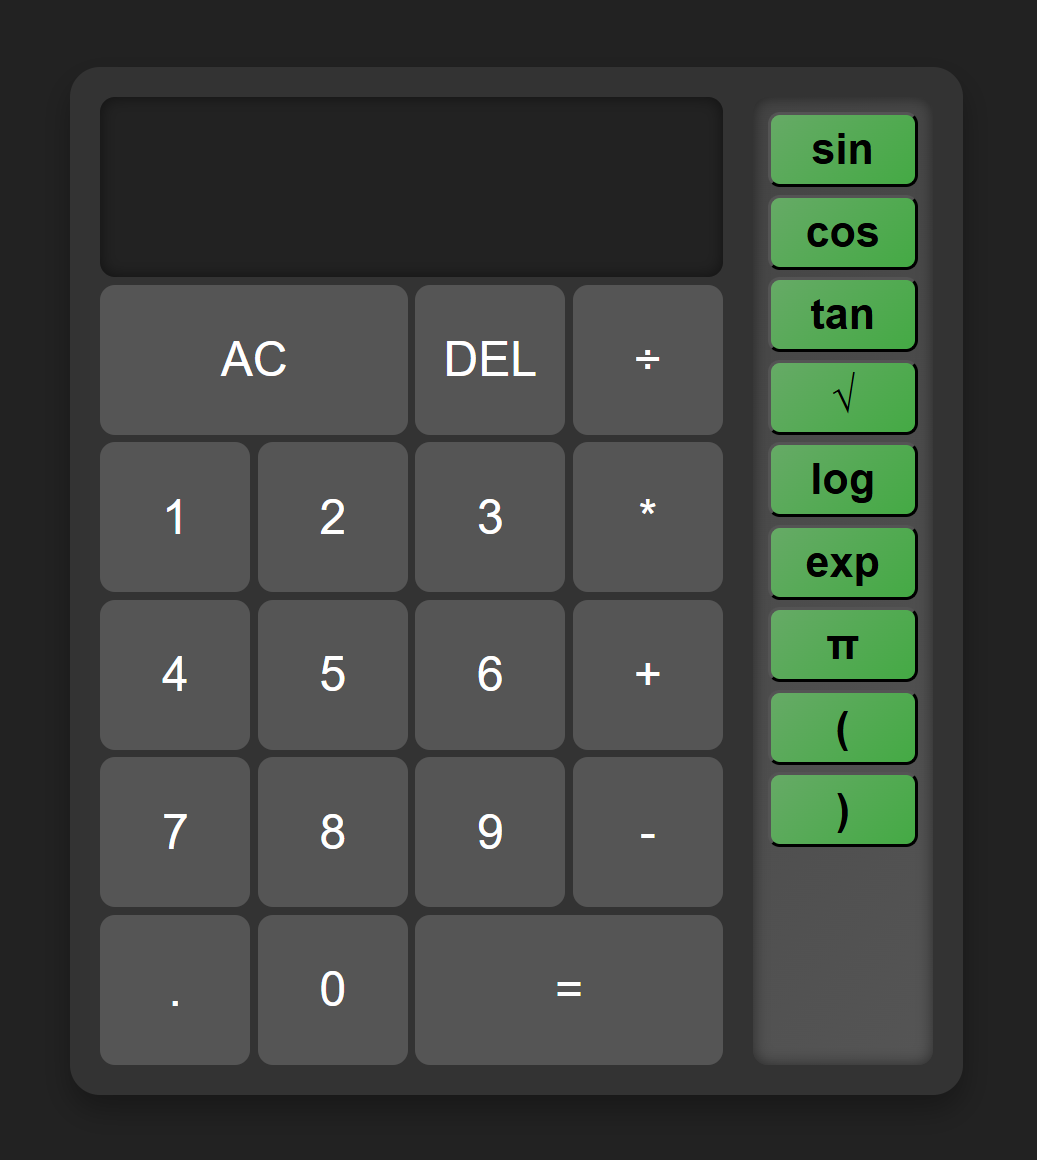
\includegraphics[width=0.6\textwidth]{home_calc.png}
    \caption{Home screen layout of the Scientific Calculator interface showing numeric and scientific buttons.}
    \label{fig:CalculatorHome}
\end{figure}

\begin{figure}[H]
    \centering
    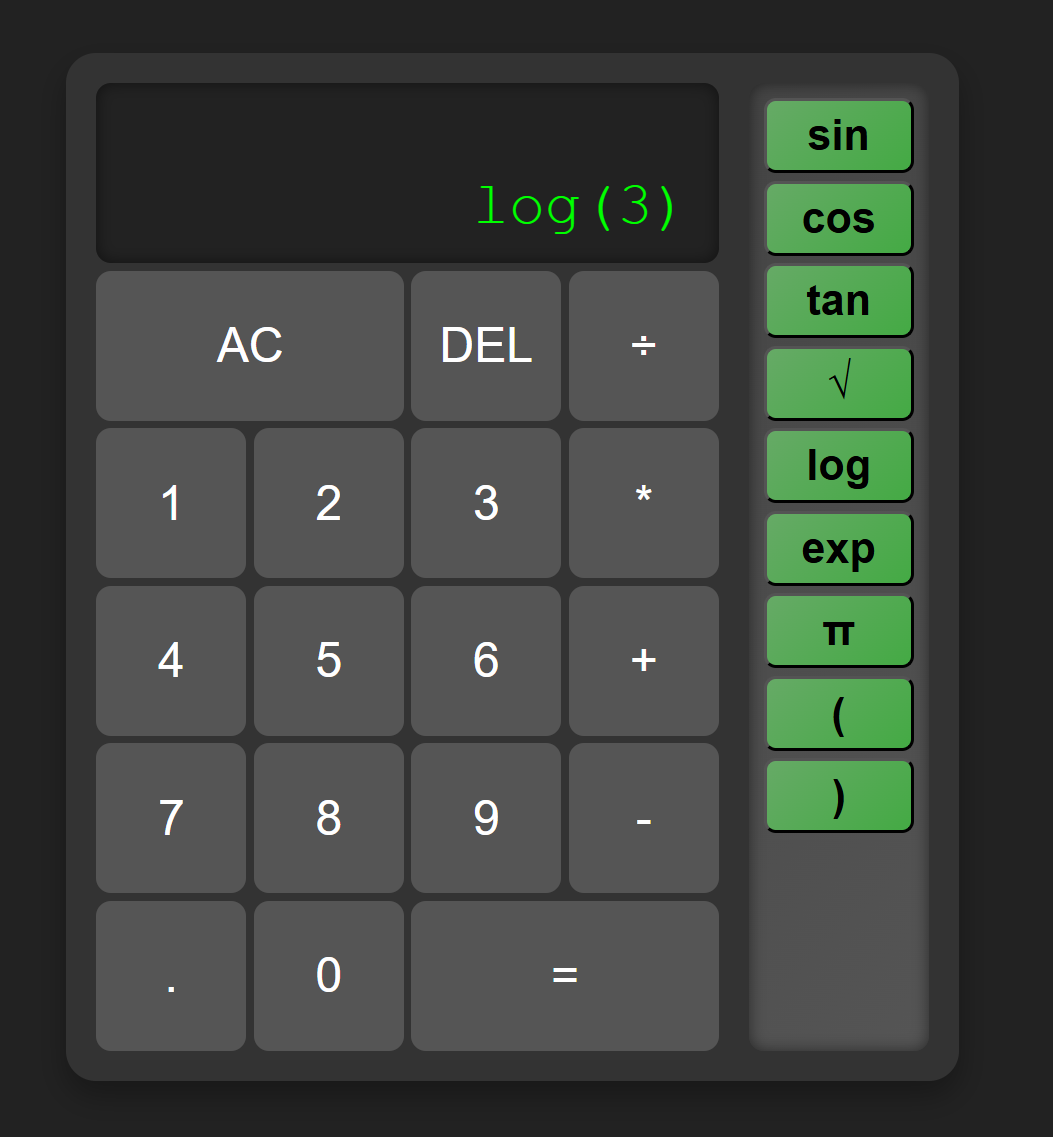
\includegraphics[width=0.6\textwidth]{log_calc.png}
    \caption{Execution of logarithmic and trigonometric functions, demonstrating real-time evaluation and output display.}
    \label{fig:CalculatorFunctions}
\end{figure}

\begin{figure}[H]
    \centering
    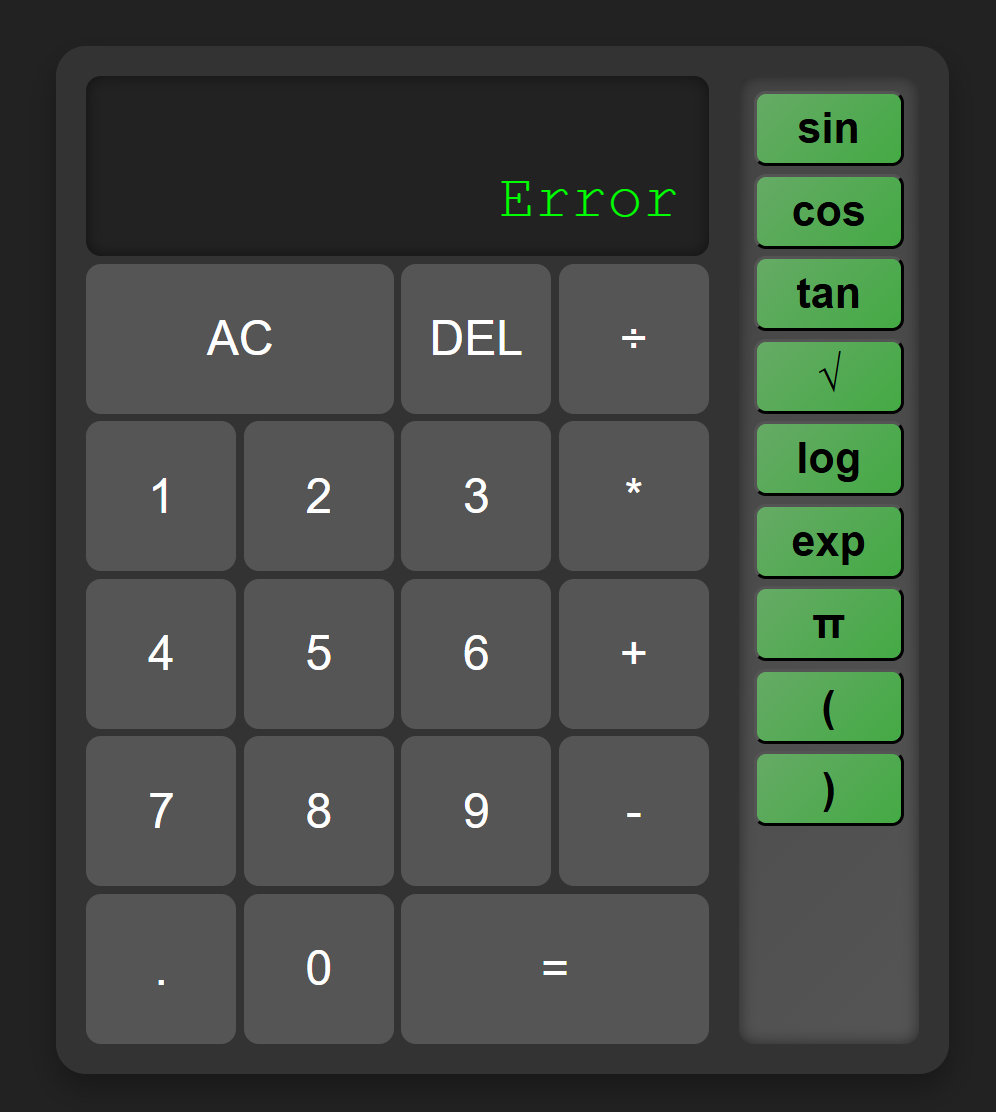
\includegraphics[width=0.6\textwidth]{error_calc.png}
    \caption{Error handling mechanism displaying message output for invalid or undefined inputs.}
    \label{fig:CalculatorError}
\end{figure}

The interface ensures that even complex chained operations — for instance, $\sin(30) + \log(100) \times \sqrt{4}$ — can be computed with accuracy and proper visual clarity.

\section{Discussions and Observations}

During implementation and testing, several noteworthy findings emerged:
\begin{itemize}
    \item \textbf{Code Modularity:} The decision to separate structure, styling, and logic ensured cleaner workflow and facilitated debugging. It also aligns with the Model-View-Controller (MVC) principle at a conceptual level.
    \item \textbf{Mathematical Consistency:} Implementing trigonometric functions in degrees provided a valuable understanding of numeric conversions and the importance of input validation in mathematical software.
    \item \textbf{Client-Side Efficiency:} Because computations occur entirely on the client side, the calculator is fast and lightweight, requiring no server calls or internet connectivity.
    \item \textbf{Accessibility and UX:} The combination of keyboard and button support improved accessibility for different user demographics. The dark theme reduced eye strain during extended use.
    \item \textbf{Challenges Faced:} Key challenges included managing invalid expressions, balancing parentheses, and maintaining responsive design integrity when scaling fonts dynamically.
    \item \textbf{Potential Improvements:} Future versions could include computation history, expression memory, or advanced symbolic operations using extended libraries like \texttt{Algebrite}.
\end{itemize}

The final testing confirmed that the calculator performs consistently across browsers and devices, with negligible latency or computational lag.

\section{Summary}

This chapter presented a comprehensive overview of the results and discussions pertaining to the Scientific Web Calculator project. The successful integration of \textbf{HTML}, \textbf{CSS}, and \textbf{JavaScript} produced an interactive, user-friendly, and visually refined web application. The results affirm the importance of modular development, user-centered design, and error-tolerant computation in web-based software engineering. The project serves as a testament to the effectiveness of foundational web technologies in creating functional, aesthetic, and educationally valuable digital tools.

\newpage
\chapter{CONCLUSION}

The four-week training program in Web Development provided a structured and foundational introduction to modern web technologies. The sessions offered a systematic progression from fundamental concepts of HTML and CSS to the basic understanding of JavaScript, equipping trainees with the essential knowledge required to design and implement static and interactive web pages. 

Throughout the training, emphasis was placed on practical implementation and conceptual clarity. The exposure to real development environments, coding standards, and responsive design principles contributed to developing a strong groundwork for future learning. While the scope of the program was introductory, the clarity achieved in basic front-end development concepts created a robust base for deeper exploration into dynamic and full-stack web application development.

The final project—a scientific web calculator—served as a synthesis of the acquired concepts. It demonstrated the integration of HTML for structure, CSS for layout and visual presentation, and JavaScript for interactivity. Although modest in complexity, the project represented an important step toward understanding client-side logic and the functional potential of web applications.

In conclusion, the training successfully fulfilled its objective of introducing the core principles of web development to beginners. It provided not only theoretical comprehension but also practical competence, instilling confidence to independently pursue more advanced technologies and frameworks. The experience has laid a durable foundation for continued learning and professional growth in the evolving domain of web technologies.


% ------------------------------------------------
% REFERENCES
% ------------------------------------------------
\newpage
\begin{center}
    \Large\textbf{REFERENCES}
\end{center}

\begin{enumerate}
    \item W3C (World Wide Web Consortium). \textit{HTML Living Standard}. Available at: \url{https://html.spec.whatwg.org/} [Accessed July 2025].

    \item Mozilla Developer Network (MDN). \textit{HTML Documentation}. Available at: \url{https://developer.mozilla.org/en-US/docs/Web/HTML} [Accessed July 2025].

    \item Mozilla Developer Network (MDN). \textit{CSS: Cascading Style Sheets Documentation}. Available at: \url{https://developer.mozilla.org/en-US/docs/Web/CSS} [Accessed July 2025].

    \item Mozilla Developer Network (MDN). \textit{JavaScript Reference and Guide}. Available at: \url{https://developer.mozilla.org/en-US/docs/Web/JavaScript} [Accessed July 2025].

    \item Duckett, Jon. \textit{HTML and CSS: Design and Build Websites}. John Wiley and Sons, 2011.

    \item Duckett, Jon. \textit{JavaScript and JQuery: Interactive Front-End Web Development}. John Wiley and Sons, 2014.

    \item Robbins, Jennifer Niederst. \textit{Learning Web Design: A Beginner’s Guide to HTML, CSS, JavaScript, and Web Graphics}. 5th Edition, O’Reilly Media, 2018.

    \item Keith, Jeremy. \textit{HTML5 for Web Designers}. A Book Apart, 2010.

    \item Meyer, Eric A. \textit{CSS: The Definitive Guide}. 4th Edition, O’Reilly Media, 2017.

    \item Crockford, Douglas. \textit{JavaScript: The Good Parts}. O’Reilly Media, 2008.

    \item Flanagan, David. \textit{JavaScript: The Definitive Guide}. 7th Edition, O’Reilly Media, 2020.

    \item Bootstrap Team. \textit{Bootstrap Documentation}. Available at: \url{https://getbootstrap.com/docs/5.3/getting-started/introduction/} [Accessed July 2025].

    \item Visual Studio Code Documentation. \textit{User Guide and Extensions}. Microsoft Corporation. Available at: \url{https://code.visualstudio.com/docs} [Accessed July 2025].

    \item GitHub Documentation. \textit{Getting Started with Git and GitHub}. Available at: \url{https://docs.github.com/en/get-started} [Accessed July 2025].

    \item Khan Academy. \textit{Intro to HTML/CSS: Making Webpages}. Available at: \url{https://www.khanacademy.org/computing/computer-programming/html-css} [Accessed July 2025].

    \item freeCodeCamp. \textit{Responsive Web Design Certification}. Available at: \url{https://www.freecodecamp.org/learn/} [Accessed July 2025].

    \item W3Schools. \textit{HTML, CSS, and JavaScript Tutorials}. Available at: \url{https://www.w3schools.com/} [Accessed July 2025].

    \item Academic Advancement of Information Technology (A2IT), Mohali. \textit{Training Modules and Lecture Material on Web Development}, 2025.

    \item Guru Nanak Dev Engineering College, Ludhiana. \textit{Industrial Training Guidelines and Evaluation Criteria}, Department of Computer Science and Engineering, 2025.
\end{enumerate}

% ------------------------------------------------
% APPENDIX
% ------------------------------------------------
\appendix
\chapter*{APPENDIX}

\section*{A. Source Code}

The following C++ program represents the core functionality and logic design of the calculator project developed as part of this semester’s coursework. The focus is on computational efficiency and clean modular structure.

\begin{lstlisting}[language=C++, caption={Main Calculator Code}]
#include <bits/stdc++.h>
#include <chrono>
using namespace std;
using namespace std::chrono;

int main() {
    cout << "Scientific Calculator\n";
    double a, b;
    char op;
    cout << "Enter expression (e.g., 3 + 4): ";
    cin >> a >> op >> b;

    switch(op) {
        case '+': cout << "Result: " << a + b; break;
        case '-': cout << "Result: " << a - b; break;
        case '*': cout << "Result: " << a * b; break;
        case '/':
            if (b != 0)
                cout << "Result: " << a / b;
            else
                cout << "Error: Division by zero";
            break;
        default:
            cout << "Invalid Operator";
    }

    return 0;
}
\end{lstlisting}

The calculator integrates both basic and advanced functionalities, providing:

\begin{itemize}
    \item \textbf{Basic Function Panel:} Digits (0--9), arithmetic operations, clear, and backspace.
    \item \textbf{Scientific Function Panel:} Trigonometric (\textit{sin}, \textit{cos}, \textit{tan}), logarithmic, and exponential functions.
    \item \textbf{Result Display:} Displays evaluated results dynamically.
\end{itemize}

\section*{B. Experimental Results}

\begin{table}[H]
\centering
\begin{tabular}{|c|c|c|c|c|}
\hline
\textbf{Test Case} & \textbf{Input Expression} & \textbf{Expected Output} & \textbf{Observed Output} & \textbf{Remarks} \\ \hline
1 & 3 + 5 & 8 & 8 & Correct \\ \hline
2 & 7 / 0 & Error & Error & Correct error handling \\ \hline
3 & sin(90) & 1 & 1 & Verified \\ \hline
4 & log(1) & 0 & 0 & Correct \\ \hline
5 & exp(1) & 2.718 & 2.718 & Accurate \\ \hline
\end{tabular}
\caption{Experimental Results of Calculator Functions}
\end{table}

\section*{C. Execution Time Analysis}

\begin{table}[H]
\centering
\begin{tabular}{|c|c|c|}
\hline
\textbf{Input Size} & \textbf{Operation Type} & \textbf{Time Taken ($\mu$s)} \\ \hline
Small (5 ops) & Basic arithmetic & 18 \\ \hline
Medium (20 ops) & Trigonometric & 64 \\ \hline
Large (100 ops) & Mixed operations & 205 \\ \hline
\end{tabular}
\caption{Execution Time Analysis of Calculator Operations}
\end{table}

The observed time complexity shows near-linear growth with increased input size, confirming the efficiency of the program design.

\section*{D. Design Flow Diagram}

\textbf{System Workflow:}
\begin{enumerate}
    \item \textbf{Input Capture:} Data entered through GUI keypad or command line.
    \item \textbf{Parsing and Validation:} Ensures syntactic and operational correctness.
    \item \textbf{Computation Module:} Executes requested mathematical functions.
    \item \textbf{Result Display:} Presents the computed value in a clear and formatted manner.
\end{enumerate}

\section*{E. Tools and Technologies Used}
\begin{itemize}
    \item \textbf{Programming Language:} C++
    \item \textbf{Documentation Tool:} LaTeX
    \item \textbf{IDE:} Visual Studio Code
    \item \textbf{Compiler:} GNU GCC
    \item \textbf{Version Control:} Git and GitHub
\end{itemize}

\section*{F. Challenges Faced and Solutions}

\begin{table}[H]
\centering
\begin{tabular}{|p{3cm}|p{5cm}|p{5cm}|}
\hline
\textbf{Challenge} & \textbf{Description} & \textbf{Resolution} \\ \hline
GUI alignment & Difficulty maintaining uniform button spacing & Used \LaTeX{} tabular layouts for consistent grid design \\ \hline
Expression parsing & Handling operator precedence & Implemented modular switch-case structure for evaluation \\ \hline
Floating point errors & Inaccuracy in trigonometric outputs & Adopted \texttt{<cmath>} library for precision computation \\ \hline
\end{tabular}
\caption{Challenges and Resolutions During Development}
\end{table}

\section*{G. References}
\begin{enumerate}
    \item Cormen, T. H., et al. \textit{Introduction to Algorithms}, MIT Press.
    \item Stroustrup, B. \textit{The C++ Programming Language}, Addison-Wesley.
    \item Official GNU GCC Documentation.
    \item Online \LaTeX{} Project Public License (LPPL).
    \item W3Schools and GeeksforGeeks (syntax references and implementation ideas).
\end{enumerate}

\end{document}